\documentclass{article}
\usepackage[most]{tcolorbox}
\usepackage{amsmath}
\usepackage{pgfplots}
\usepackage{pgfplotstable}

\begin{document}




\vspace{20pt}

\begin{tcolorbox}[colback=blue!5!white,colframe=blue!75!black,title=Question 13]
The function \( f \) is defined by:

\[
f(x) = ax^2 + bx + c
\]

where \( a, b, \) and \( c \) are constants. The graph of \( y = f(x) \) in the xy-plane passes through the points \( (8,0) \) and \( (-2,0) \). If \( a \) is an integer greater than 1, which of the following could be the value of \( a + b \)?

\begin{itemize}
    \item[A.] -10
    \item[B.] -5
    \item[C.] 6
    \item[D.] 7
\end{itemize}
\end{tcolorbox}

\begin{tcolorbox}[colback=green!10, colframe=green!50!black,title=Answer to Question 13]
\textbf{Correct Answer: A}  
\end{tcolorbox}

\vspace{20pt}

\begin{tcolorbox}[colback=blue!5!white,colframe=blue!75!black,title=Question 14]
The given equation is one equation in a system of two linear equations. If the system of equations has \textbf{at least one solution}, which of the following equations could be the other equation in the system?

\[
7x + 5y = 2
\]

\begin{itemize}
    \item[I.] \( 10.5x + 7.5y = 3 \)
    \item[II.] \( 10.5x - 7.5y = 3 \)
\end{itemize}

\begin{itemize}
    \item[A.] I only
    \item[B.] II only
    \item[C.] I and II
    \item[D.] Neither I nor II
\end{itemize}
\end{tcolorbox}

\begin{tcolorbox}[colback=green!10, colframe=green!50!black,title=Answer to Question 14]
\textbf{Correct Answer: C}  
\end{tcolorbox}

\vspace{20pt}

\begin{tcolorbox}[colback=blue!5!white,colframe=blue!75!black,title=Question 15]
Each of the following frequency tables represents a data set. Which of these frequency tables represents the data set with the smallest standard deviation?

\begin{itemize}
    \item[A.]
    \begin{tabular}{|c|c|}
    \hline
    Value & Frequency \\
    \hline
    5  & 0  \\
    6  & 10  \\
    7  & 55  \\
    8  & 10  \\
    \hline
    \end{tabular}
    
    \item[B.]
    \begin{tabular}{|c|c|}
    \hline
    Value & Frequency \\
    \hline
    5  & 11  \\
    6  & 17  \\
    7  & 19  \\
    8  & 17  \\
    9  & 11  \\
    \hline
    \end{tabular}
    
    \item[C.]
    \begin{tabular}{|c|c|}
    \hline
    Value & Frequency \\
    \hline
    5  & 15  \\
    6  & 15  \\
    7  & 15  \\
    8  & 15  \\
    9  & 15  \\
    \hline
    \end{tabular}

        \item[D.]
    \begin{tabular}{|c|c|}
    \hline
    Value & Frequency \\
    \hline
    5  & 16  \\
    6  & 17  \\
    7  & 18  \\
    8  & 18  \\
    9  & 16  \\
    \hline
    \end{tabular}
\end{itemize}
\end{tcolorbox}

\begin{tcolorbox}[colback=green!10, colframe=green!50!black,title=Answer to Question 15]
\textbf{Correct Answer: A}  
\end{tcolorbox}

\vspace{20pt}

\begin{tcolorbox}[colback=blue!5!white,colframe=blue!75!black,title=Question 16]
Ari will add a 135-year-old stamp to her original collection, creating a new collection of 52 stamps.

\begin{center}
\begin{tabular}{|c|c|}
\hline
Age & Frequency \\
\hline
80  & 5  \\
85  & 6  \\
90  & 5  \\
95  & 10  \\
\hline
Total & 51 \\
\hline
\end{tabular}
\end{center}

Which statement correctly compares the mean ages and median ages of Ari’s original and new collections?

\begin{itemize}
    \item[A.] The mean age for the new collection is greater than the mean age for the original collection, and the median age for the new collection is greater than the median age for the original collection.
    \item[B.] The mean age for the new collection is greater than the mean age for the original collection, but the median age is the same for the original and new collections.
    \item[C.] The mean age for the new collection is less than the mean age for the original collection, and the median age for the new collection is less than the median age for the original collection.
    \item[D.] The median age for the new collection is greater than the median age for the original collection, but the mean age is the same for the original and new collections.
\end{itemize}
\end{tcolorbox}

\begin{tcolorbox}[colback=green!10, colframe=green!50!black,title=Answer to Question 16]
\textbf{Correct Answer: 
}  
\end{tcolorbox}


\begin{tcolorbox}[colback=blue!5!white,colframe=blue!75!black,title=Question]
Two teachers kept track of how much time each student in their homeroom class spent volunteering last month. These box plots show the results.

\begin{center}
    \textbf{Hours Spent Volunteering}
    
    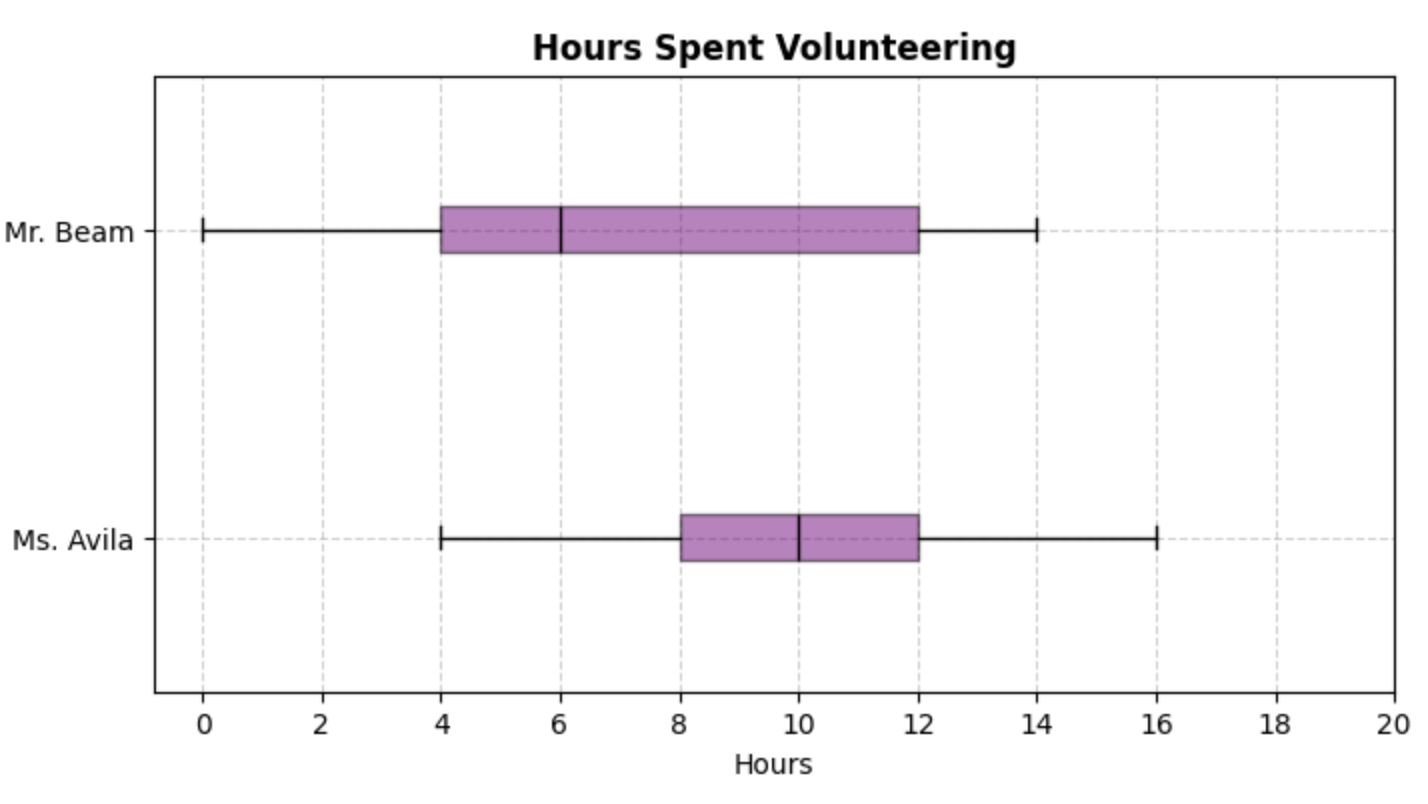
\includegraphics[width=0.8\textwidth]{F5.png} % Replace with actual image if needed
\end{center}

Based on the data in the box plots, determine which statement is true?

\begin{itemize}
    \item[(A)] The student who volunteered the least number of hours is in Ms. Avila's class.
    \item[(B)] Students in Ms. Avila's class generally spent less time volunteering than students in Mr. Beam's class did.
    \item[(C)] The IQR in the amount of time students in Ms. Avila's class spent volunteering is less than the amount of time students in Mr. Beam's class spent volunteering.
    \item[(D)] One fourth of all the students in the two classes combined volunteered for at least 12 hours.
\end{itemize}

\end{tcolorbox}



\begin{tcolorbox}[colback=green!10, colframe=green!50!black,title=Answer to Question ]
\textbf{Correct Answer: C
}  
\end{tcolorbox}

\begin{tcolorbox}[colback=blue!10, colframe=blue!50!black, title=Question 18]
In a set of four consecutive odd integers, where the integers are ordered from least to greatest, the first integer is represented by \( x \). The product of 28 and the third odd integer in the set is at most the value of 50 less than the sum of the first and fourth odd integers in the set. What is the greatest possible value of \( x \)?

\begin{itemize}
    \item[A.] \( -5 \)
    \item[B.] \( -6 \)
    \item[C.] \( -7 \)
    \item[D.] \( -8 \)
\end{itemize}
\end{tcolorbox}

\begin{tcolorbox}[colback=green!5!white, colframe=green!75!black, title=Solution]
The four consecutive odd integers are: \( x, x+2, x+4, x+6 \).  
The third odd integer is \( x+4 \), and the given condition states:

\[
28(x+4) \leq (x + x + 6) - 50
\]

\[
28x + 112 \leq 2x + 6 - 50
\]

\[
28x + 112 \leq 2x - 44
\]

\[
26x \leq -156
\]

\[
x \leq -6
\]

Since \( x \) must be an odd integer, the greatest possible value is \( -7 \).
\end{tcolorbox}

\vspace{1cm}

\begin{tcolorbox}[colback=blue!10, colframe=blue!50!black, title=Question 12]
In the given equation, \( c \) is a constant. A solution to the equation is 

\[
\frac{-27 + \sqrt{261}}{26}
\]

What is the value of \( c \)?

\[
x(13x + 27) + c = 5
\]

\begin{itemize}
    \item[A.] 14 
    \item[B.] 9
    \item[C.] 5
    \item[D.] 4
\end{itemize}
\end{tcolorbox}

\begin{tcolorbox}[colback=green!5!white, colframe=green!75!black, title=Solution]
Using the quadratic formula:

\[
x = \frac{-b \pm \sqrt{b^2 - 4ac}}{2a}
\]

Rewriting the equation:

\[
13x^2 + 27x + c - 5 = 0
\]

Since:

\[
\sqrt{b^2 - 4ac} = \sqrt{261}
\]

\[
27^2 - 4(13)(c - 5) = 261
\]

\[
729 - 52c + 260 = 261
\]

\[
989 - 52c = 261
\]

\[
52c = 728
\]

\[
c = 14
\]
\end{tcolorbox}

\vspace{1cm}

\begin{tcolorbox}[colback=blue!10, colframe=blue!50!black, title=Question 21]
The function \( h(x) \) is defined as:

\[
h(x) = -\sqrt{x^2 + bx + c}
\]

where \( b \) and \( c \) are constants. The graph of \( y = h(x) \) contains the points \( (2,0) \) and \( (0, -\sqrt{358}) \). If \( h(m) = 0 \), what is the greatest possible value of \( m \)?

\begin{itemize}
    \item[A.] 2
    \item[B.] 177
    \item[C.] 179 
    \item[D.] 358
\end{itemize}
\end{tcolorbox}

\begin{tcolorbox}[colback=green!5!white, colframe=green!75!black, title=Solution]
Since \( h(2) = 0 \), we substitute:

\[
0 = -\sqrt{2^2 + 2b + c}
\]

\[
\Rightarrow \sqrt{4 + 2b + c} = 0
\]

\[
4 + 2b + c = 0
\]

\[
c = -4 - 2b
\]

Since \( h(0) = -\sqrt{358} \), we substitute:

\[
-\sqrt{358} = -\sqrt{0^2 + 0b + c}
\]

\[
\Rightarrow \sqrt{c} = \sqrt{358}
\]

\[
c = 358
\]

From \( c = -4 - 2b \), we get:

\[
358 = -4 - 2b
\]

\[
2b = -4 - 358
\]

\[
b = \frac{-362}{2} = -181
\]

The equation becomes:

\[
h(x) = -\sqrt{x^2 - 181x + 358}
\]

Setting \( h(m) = 0 \):

\[
\sqrt{m^2 - 181m + 358} = 0
\]

\[
m^2 - 181m + 358 = 0
\]

Factoring:

\[
(x-2)(x-179) = 0
\]

\[
x = 2 \quad \text{or} \quad x = 179
\]

Thus, the greatest possible value of \( m \) is \( 179 \).
\end{tcolorbox}




\begin{tcolorbox}[colback=blue!10, colframe=blue!50!black, title=Question 20]
The functions \( f \) and \( g \) are defined by the equations shown, where \( a \) and \( b \) are integer constants, \( a < b \), and \( b < 0 \). If \( y = f(x) \) and \( y = g(x) \) are graphed in the xy-plane, which of the following equations displays, as a constant or coefficient, the y-coordinate of the y-intercept of the graph of the corresponding function?

\begin{itemize}
    \item[I.] \( f(x) = a(2.1)^{x+b} \)
    \item[II.] \( g(x) = a(2.1)^x + b \)
\end{itemize}

\begin{itemize}
    \item[A.] I only
    \item[B.] II only
    \item[C.] I and II 
    \item[D.] Neither I nor II
\end{itemize}
\end{tcolorbox}

\begin{tcolorbox}[colback=green!5!white, colframe=green!75!black, title=Solution]
D.
\end{tcolorbox}

\newpage
\begin{tcolorbox}[colback=blue!5!white, colframe=blue!75!black, title=Question 21]
Right rectangular prism \(X\) is similar to right rectangular prism \(Y\).
The surface area of right rectangular prism \(X\) is \(56\) square centimeters (\(\text{cm}^2\)), and the surface area of right rectangular prism \(Y\) is \(896\) \(\text{cm}^2\).
The volume of right rectangular prism \(Y\) is \(1,536\) cubic centimeters (\(\text{cm}^3\)).
What is the sum of the volumes, in \(\text{cm}^3\), of right rectangular prism \(X\) and right rectangular prism \(Y\)?

\end{tcolorbox}

\begin{tcolorbox}[colback=green!10, colframe=green!50!black, title=Answer]
Correct answer: \(C\)

\textbf{Solution:} 

Find the ratio of the surface areas:
\[
\frac{\text{Surface Area of } Y}{\text{Surface Area of } X} = \frac{896}{56} = 16
\]

Since the prisms are similar, the ratio of their volumes is:
\[
\text{Ratio of volumes} = 16^{3/2} = 64
\]

Let \(V_X\) be the volume of \(X\), so:
\[
V_X = \frac{1,536}{64} = 24
\]

Sum of volumes:
\[
V_X + V_Y = 24 + 1,536 = 1,560
\]
\end{tcolorbox}

\vspace{1cm}

\begin{tcolorbox}[colback=blue!5!white, colframe=blue!75!black, title=Question 16]
To investigate the effect of magnesium supplementation on the sleep quality of adults, a researcher selected \(190\) adults at random from a community center to participate in a study.
Each participant was then randomly assigned to take a magnesium supplement or a placebo each day for \(6\) weeks.
At the end of the \(6\) weeks, the researcher measured the sleep efficiency of all participants again and found that the magnesium supplement caused statistically significant improved sleep quality for the adults at the community center.
What feature of this study allowed the researcher to conclude that the magnesium supplement caused the improved sleep quality?

\begin{itemize}
    \item[A.] There were more than \(100\) participants in the study.
    \item[B.] The participants were selected at random from the community center.
    \item[C.] The sleep efficiency of each participant was measured again at the end of \(6\) weeks.
    \item[D.] Each participant was randomly assigned to take a magnesium supplement or a placebo.
\end{itemize}
\end{tcolorbox}

\begin{tcolorbox}[colback=green!10, colframe=green!50!black, title=Answer]
Correct answer: \(D\)

\textbf{Solution:}

Random assignment is the key feature because it ensures that the two groups (magnesium supplement and placebo) were similar at the start of the experiment.
This means that any differences in sleep quality at the end of the study can be attributed to the magnesium supplement rather than other variables.
By randomly assigning participants to either the supplement or the placebo group, the researcher controlled for confounding variables and was able to make a causal inference.
\end{tcolorbox}

\vspace{1cm}

\begin{tcolorbox}[colback=blue!5!white, colframe=blue!75!black, title=Question 15]
For the function \( f \), for every increase of \(2\) in the value of \( x \), the value of \( f(x) \) increases by a factor of \( c \), where \( c \) is a constant.
Which of the following equivalent forms of function \( f \) displays the value of \( c \) as the base or the coefficient?

\begin{itemize}
    \item[A.] \( f(x) = 42(2)^{6x} \)
    \item[B.] \( f(x) = 42(8)^{2x} \)
    \item[C.] \( f(x) = 42(64)^x \)
    \item[D.] \( f(x) = 42(4,069)^{\frac{x}{2}} \)
\end{itemize}
\end{tcolorbox}

\begin{tcolorbox}[colback=green!10, colframe=green!50!black, title=Answer]
Correct answer: \(D\)

\end{tcolorbox}



\end{document}
